\documentclass[letterpaper]{article}
\usepackage{aaai19}
\usepackage{times}
\usepackage{helvet}
\usepackage{courier}
\usepackage[hyphens]{url}
\usepackage{graphicx}
\urlstyle{rm}
\def\UrlFont{\rm}
\usepackage{graphicx}
\frenchspacing
\setlength{\pdfpagewidth}{8.5in}
\setlength{\pdfpageheight}{11in}
% Add additional packages here.
%
% The following
% packages may NEVER be used (this list
% is not exhaustive:
% authblk, caption, CJK, float, fullpage, geometry,
% hyperref, layout, nameref, natbib, savetrees,
% setspace, titlesec, tocbibind, ulem
%
\usepackage{amsmath}
\usepackage{amsthm}
\newtheorem*{example}{Example}
\newcommand{\eg}{\mbox{\it e.g.}}
\newcommand{\name}{AI-advised human decision making}
\usepackage{enumitem}
\newtheorem*{definition}{Definition}
\newcommand{\hone}{\mbox{$h_1$}}
\newcommand{\htwo}{\mbox{$h_2$}}
\newcommand{\dtrainone}{\mbox{$D_1$}}
\newcommand{\dtraintwo}{\mbox{$D_2$}}
\newcommand{\compatscore}{\mathcal{C}}
\newcommand{\loss}{L}
\newcommand{\lossbc}{\loss_c}
\newcommand{\lambdabc}{\lambda_c}
\newcommand{\dissonance}{\mathcal{D}}
\newcommand{\ie}{\mbox{\it i.e.}}
\usepackage{bbm}
\newcommand{\plat}{{\sc Caja}}
\usepackage{subcaption}
\newcommand{\err}{\textit{err}}
\newcommand{\etal}{\mbox{\it et al.}}

%
% PDFINFO
% You are required to complete the following
% for pass-through to the PDF.
% No LaTeX commands of any kind may be
% entered. The parentheses and spaces
% are an integral part of the
% pdfinfo script and must not be removed.
%
\pdfinfo{
/Title (Updates in Human-AI Teams: The Performance/Compatibility Tradeoff)
/Author (Gagan Bansal, Besmira Nushi, Ece Kamar, Daniel S. Weld, Walter S. Lasecki, Eric Horvitz)
}
%
% Section Numbers
% Uncomment if you want to use section numbers
% and change the 0 to a 1 or 2
% \setcounter{secnumdepth}{0}
% Title and Author Information Must Immediately Follow
% the pdfinfo within the preamble
%
\title{Updates in Human-AI Teams:\\ Understanding and Addressing the Performance/Compatibility Tradeoff}
\author{Gagan Bansal,\textsuperscript{\rm 1} Besmira Nushi,\textsuperscript{\rm 2} Ece Kamar,\textsuperscript{\rm 2} Daniel S. Weld,\textsuperscript{\rm 1} Walter S. Lasecki,\textsuperscript{\rm 3} Eric Horvitz\textsuperscript{\rm 2}\\
\textsuperscript{\rm 1}University of Washington,
\textsuperscript{\rm 2}Microsoft Research,
\textsuperscript{\rm 3}University of Michigan
}

 %
\begin{document}
\maketitle
\begin{abstract}
AI systems are being deployed to support human decision making in high-stakes domains such as healthcare and criminal justice. In many cases, the human and AI form a team, in which the human makes decisions after reviewing the AI's inferences. A successful partnership requires that the human develops insights into the performance of the AI system, including its failures. We study the influence of {\em updates} to an AI system in this setting. While updates can increase the AI's predictive performance, they may also lead to behavioral changes that are at odds with the user's prior experiences and confidence in the AI's inferences. We show that updates that increase AI performance may actually hurt {\em team} performance. 
We introduce the notion of the {\em compatibility} of an AI update with prior user experience and present methods for studying the role of compatibility in human-AI teams. 
Empirical results on three high-stakes classification tasks show that current machine learning algorithms do not produce compatible updates. We propose a re-training objective to improve the compatibility of an update by penalizing new errors. The objective offers full leverage of the performance/compatibility tradeoff across different datasets, enabling more compatible yet accurate updates.
\end{abstract}

\section{Introduction}

A promising opportunity in AI is developing systems that can partner with people to accomplish tasks in ways that exceed the capabilities of either individually~\cite{wang2016deep,kamar2016directions,gaur2016effects}.
We see many motivating examples: a doctor using a medical expert system~\cite{wang2016deep}, a judge advised by a recidivism predictor, or a driver supervising a semi-autonomous vehicle. Indeed, economists expect human-AI teams to handle many such tasks~\cite{forrester-17}. Despite rising interest, there is much to learn about creating effective human-AI teams and what capabilities AI systems should employ to be competent partners. 

\begin{figure}[t]
    \begin{center}
    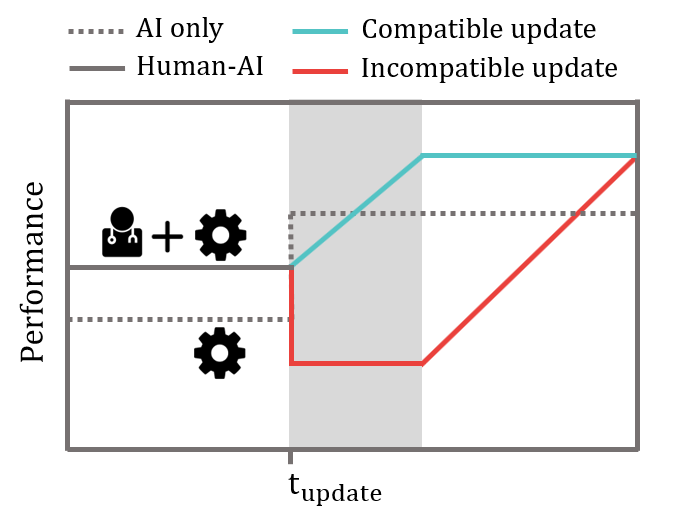
\includegraphics[width=\linewidth]{Picture1v2.png}
    \end{center}
    \caption{Schematized view of human-AI teams in the presence of AI updates. Human-AI teams perform better than either alone, but when the AI is {\em updated} its behavior may violate human expectations. Even if updates increase the AI's {\em individual} performance, they may reduce {\em team} performance by making mistakes in regions where humans have learned to trust the AI.}
    \label{fig:landing}
\end{figure}

We study human-AI teams in decision-making settings where a user takes action recommendations from an AI partner for solving a complex task. The user considers the recommendation and, based on previous experience with the system, decides to accept the suggested action or take a different action. We call this type of interaction {\em AI-advised human decision making}. While there exist other important forms of human-AI collaboration (including human-advised AI decision making and more general collaborative decision making involving a mix of initiatives and emergent team behaviors), we focus on a specific interplay where the goal is to create AI systems that recommend actions to assist humans with decisions in high-stakes domains~\cite{angwin2016machine,bayati2014data}. The motivation for AI-advised human decision making comes from the fact that humans and machines have complementary strengths and abilities. While both human experts and machine-learned models are not perfect on a task like medical diagnosis or object classification, researchers have shown that their ideal combination could significantly improve performance~\cite{wang2016deep,kamar2012combining}. 
AI systems offer added benefits by speeding up decision making when humans can identify tasks where the AI can be trusted and no more human effort is needed~\cite{lasecki2012scribe,lasecki2012real}. 

It might be expected that improvements in the performance of AI systems lead to stronger team performance, but, as with human groups, individual ability is only one of many factors that affect team effectiveness~\cite{dechurch-jap10,grosz1996collaborative}. Even in a simple collaboration scenario, in which an AI system assists a human decision maker with predictions, the success of the team hinges on the human correctly deciding when to follow the recommendation of the AI system and when to override. Unless the particular domain and the interaction allows the human to validate the correctness of the machine recommendation efficiently and effectively, extracting benefits from collaboration with the AI system depends on the human developing insights (i.e., a mental model) of when to trust the AI system with its recommendations. If the human mistakenly trusts the AI system in regions where it is likely to err, catastrophic failures may occur. 
Human-AI teams become especially susceptible to such failures because of discrepancies introduced by system updates that do not account for human expectations. The following example and Figure~\ref{fig:landing} illustrate this situation.


\begin{example}[\sc{Patient readmission}]
A doctor uses an AI system that is 95\% accurate at predicting whether a patient will be readmitted following their discharge to make decisions about enlisting the patient in a supportive post-discharge program. The special program is costly but promises to reduce the likelihood of readmission. After a year of interacting with the AI, the doctor develops a clear mental model that suggests she can trust the AI-advised actions on elderly patients. In the meantime, the AI's developer trains and deploys a new 98\% accurate classifier, which errs on elderly patients. 
While the AI has improved by 3\%, the doctor is unaware of the new errors, and as a result of this outdated mental model, takes the wrong actions for some elderly patients.
\end{example}

This example is motivated by real-world AI applications for reducing patient readmissions and other costly outcomes in healthcare~\cite{bayati2014data,wiens2016patient,caruana2015intelligible}, and motivates the need for reducing the cost of disruption caused by updates that violate  %incompatible with 
users' mental models. The problem with updates extends to numerous AI-advised human decision-making settings; similar challenges have been observed during over-the-air updates in the Tesla autopilot,\footnote{\url{www.theverge.com/2018/6/2/17413732/tesla-over- the-air-software-updates-brakes.}} and  analogous issues arise in a variety of other settings when AI services 
being consumed by third-party applications, are updated.

Despite these problems, developers have almost exclusively optimized for AI performance.  Retraining techniques largely ignore important details about human-AI teaming, and the mental model that humans develop from interacting with the system. %  faithful to previous successful human-AI interactions. 
The goal of this work is to make the human factor a first-class consideration of AI updates. We make the following contributions: 

\begin{itemize}
\item We define the notion of compatibility of an AI update with the user's mental model created from past experience.
We then propose a practical adjustment to current ML (re)training algorithms --- an additional differentiable term to the logarithmic loss --- that improves compatibility during updates, 
and allows developers to explore the performance/compatibility tradeoff.

\item We introduce an open-source experimental platform\footnote{Available at \url{https://github.com/gagb/caja}} for 
studying how people model the error boundary of an AI teammate in the presence of updates for a an AI-advised decision-making task. %Since it is challenging to study human mental models, 
The platform exposes important design factors (\eg, task complexity, reward, update type) to the experimenter. 

\item Using the platform, we perform user studies showing that, humans develop mental models of AI systems across different conditions, and that more accurate mental models improve team performance. More importantly, we show that updating an AI to increase accuracy, at the expense of compatibility, may {\em degrade} team performance. 
 Moreover, experiments on three high-stakes classification tasks (recidivism prediction, in-hospital mortality prediction, and credit-risk assessment) demonstrate that: (i) current ML models are not inherently compatible, but (ii) flexible performance/compatibility tradeoffs can be effectively achieved via a reformulated training objective.


\end{itemize}


\section{AI-Advised Human Decision Making}

In our studies, we focus on a simple, but common, model of human-AI teamwork that abstracts many real-world settings,
\eg, a 30-day readmission classifier supporting a doctor~\cite{bayati2014data}, a recidivism predictor supporting judges in courts~\cite{angwin2016machine}. In this setting, which we call {\em \name}, an AI 
system provides a {\em recommendation}, but the human makes the final {\em decision}.
The team solves a sequence of tasks, repeating the following cycle for each time, $t$.

\begin{itemize}[leftmargin=.25in]
\item[S1:] The environment provides an input, $x^t$. 
\item[S2:] The AI (possibly mistaken) suggests an action, $h(x^t)$. 
\item[S3:] Based on this input, the human makes her decision, $u^t$.
\item[S4:] The environment returns a reward, $r^t$, which is a function of the user's action, the (hidden) best action, and other costs of the human's decision (e.g., time taken).
\end{itemize}

\noindent While interacting over multiple tasks, the team receives repeated feedback about performance, which lets the human learn when she can trust the AI's answers. The cumulative reward $R$ over $T$ cycles records the team's performance.


\subsection{Trust as a Human's Mental Model of the AI}

\noindent Cognitive psychology research shows that when people interact with any complex system, they create a mental model, which facilitates their use of the system~\cite{donald1988psychology}. Just as for other automated systems, humans create a mental model of AI agents~\cite{kulesza2012tell}.
In \name, valid mental models of the reliability of the AI output improve collaboration by helping the user to know when to trust the AI's recommendation.
A perfect mental model of the AI system's reliability could be harnessed to achieve the highest team performance. A simple definition for such a model would be $m: x \rightarrow \{T, F\}$, indicating which inputs the human trusted the AI to solve correctly. A more complex model might compute a probability and include additional arguments, such as  the AI's output, $h(x).$
In reality, mental models are not perfect \cite{norman2014some}: users develop them through limited interaction with the system, and people have cognitive limitations.
Furthermore, different team members may have access to different information about the situation. 
For example, a doctor may know things about a patient that are missing from electronic health records (\eg, an estimate of the patient's compliance with taking medications), while an AI system may have access to the most recent results and trends in physiological state that are not tracked by physicians. 
In summary, users learn and evolve a model of an AI system's competence over the course of many interactions. In the experimental section, we show that these models can greatly improve team performance. Next, we study the problem of updating an AI system within the context of AI-assisted human decision making, and introduce the notion of compatibility.

\section{Compatibility of Updates to Classifiers}

Developers regularly update AI systems by training new models with additional or higher-quality training data, or by switching to an improved learning algorithm. 
Such updates presumably improve the AI's performance on a validation set, but the patient readmission example highlights how this is not always sufficient: updates can arbitrarily change the AI's error boundary, introduce new errors which violate user expectations and decrease team performance.

In software engineering, an update is \emph{backward compatible} if the updated system can support legacy software.
By analogy, we define that an update to an AI component is {\em locally compatible} with a user's mental model if it does not introduce new errors and the user, even after the update, can safely trust the AI's recommendations. 


\begin{definition}[\textsc{Locally-Compatible Update}]
Let $m(x)$ denote a mental model that dictates the user's trust of the AI on input $x$.  Let $A(x,u)$ denote whether $u$ is the appropriate action for input $x$. 
An update, \htwo, to a learned model, \hone, is locally compatible with $m$ iff 
\[\forall x, [m(x) \wedge A(x, \hone(x))] \Rightarrow A(x, \htwo(x)) \]
\end{definition}

In other words, an update is compatible only if, for every input where the user trusts the AI and \hone\ recommends the correct action, the updated model, \htwo, also recommends the correct action. In the rest of this paper, we focus on situations where a classifier's predictions are actions. For instance, in the patient readmission example, if a classifier predicts that the patient will be readmitted in the next 30 days, the suggested action from the classifier would be to include the patient in a special post-discharge program.

\subsection{Globally Compatible Updates}

When developers are building an AI system that is used by many individuals, it may be too difficult to track individual mental models or to deploy different updated models to different users. In this situation, an alternative to creating locally compatible updates, is a {\em globally compatible update}. To make this notion precise, we observe that a developer who is updating a classifier with new training data goes through the following steps: 

\begin{itemize}
%\setlength\itemsep{.1em}
    \item[1.] Collect initial training data $\dtrainone$.
    \item[2.] Train a model $\hone$ on $\dtrainone$ and deploy $\hone$.
    \item[3.] Collect additional data to create $\dtraintwo$, where $\dtrainone \subset \dtraintwo$.
    \item[4.] Train $\htwo$ on $\dtraintwo$.
    \item[5.] If the performance of $\htwo$ is higher than $\hone$, deploy $\htwo$.
\end{itemize}
Similar steps can be formulated for a model update where the training data does not change ($\dtraintwo=\dtrainone$) but $\htwo$ belongs to a different model class. 
\begin{definition}[\textsc{Globally-Compatible Update}]
An updated model, \htwo,  is globally compatible with \hone, iff
\[\forall x, A(x, h(x))\Rightarrow A(x, \htwo(x)) \]
\end{definition}

Note that a globally compatible update is locally compatible for {\em any} mental model.  While global compatibility is a nice ideal, satisfying it for all instances is difficult in practice. More realistically, we seek to minimize the number of errors made by \htwo's that were not made by $\hone$, since that will hopefully minimize confusion among users. 
To make this precise, we introduce the notion of a {\em compatibility score}. 

\begin{definition} [\textsc{Compatibility Score}]   
The compatibility score $\compatscore$ of an update $\htwo$ to $\hone$ is given by the fraction of examples on which $\hone$ recommends the correct action, $\htwo$ also recommends the correct action.
\begin{equation}
\label{eq:score}
    \compatscore(\hone, \htwo) =  \frac{\sum_{x}A(x, \hone(x)) \cdot A(x, \htwo(x))}{\sum_{x }A(x, \hone(x))}
\end{equation}
\end{definition}
If $\htwo$ introduces no new errors, $\compatscore(\hone, \htwo)$ will be 1. Conversely, if all the errors are new, the score will be 0. 

\subsection{Dissonance and Loss}
To train classifiers, ML developers optimize for the predictive performance of $\htwo$
by specifying, and minimizing, a classification loss $\loss$ that penalizes low performance. The equation below shows the negative logarithmic loss (also known as log loss or cross-entropy loss) for binary classification -- a commonly used training objective in ML. 
\begin{equation*}
    \label{eq:logloss}
    \loss(x, y, \htwo) = y \cdot \log p(\htwo(x)) + (1 - y) \cdot \log (1 - p(\htwo(x)))
\end{equation*}
Here, the probability $p(h(x))$ denotes the confidence of the classifier that recommendation $h(x)$ is true, while $y$ is the true label for $x$ (\ie, $A(x, y) = \mbox{\em True}$).
The negative log loss, like many other loss functions in machine learning, depends only on the true label and the confidence in prediction -- it ignores the previous versions of the classifier and, hence, has no preference for compatibility. As a result, retraining using different data can lead to very different hypotheses, introduce new errors, and decrease the compatibility score. 
To alleviate this problem, we define a new loss function $\lossbc$ expressed as the sum of classification loss and {\em dissonance}.

\begin{definition}[\textsc{Dissonance}]
The dissonance $\dissonance$ of $\htwo$ to $\hone$ is a function $\dissonance: x, y, \hone, \htwo \rightarrow \mathcal{R}$ that penalizes a low compatibility score. Furthermore, $\dissonance$ is differentiable.
\begin{equation}
    \label{eq:diss}
    \dissonance(x, y, \hone, \htwo) = \mathbbm{1}(\hone(x) = y) \cdot \loss(x, y, \htwo)
\end{equation}
\end{definition}

\noindent Recall that  $\compatscore(\hone, \htwo)$ is high when both $\hone$ and $\htwo$ are correct (Equation~\ref{eq:score}).  Dissonance  expresses the opposite notion: measuring if $\hone$ is correct ($\mathbbm{1}$ denotes an indicator function)
and penalizing by the degree to which $\htwo$ is incorrect.
Equation~\ref{eq:lossbc} defines the new loss.
\begin{equation}
    \label{eq:lossbc}
    \lossbc = \loss + \lambdabc \cdot \dissonance
\end{equation}

\noindent Here, $\lambdabc$ encodes the relative weight of dissonance, controlling the additional loss to be assigned to all new errors.
We refer to this version as {\em new-error dissonance}.
Just as with classification loss, there are other ways to realize dissonance. We explored two alternatives, which we refer to as {\em imitation} and {\em strict imitation} dissonance.
Equation~\ref{eq:diss_imitation} describes the imitation dissonance which measures the log loss between the prediction probabilities of $\hone$ and $\htwo$:
\begin{equation}
    \label{eq:diss_imitation}
    \dissonance'(x, y, \hone, \htwo) = \loss(x, \hone, \htwo)
\end{equation}

\noindent Equation~\ref{eq:diss_imitation} is used in model distillation~\cite{ba2014deep,hinton2015distilling}, where the aim is to train a shallower, less expensive model by imitating the probabilities of larger, accurate model. Unfortunately, $\dissonance'$ has the effect of nudging \htwo\ to mimic \hone's mistakes as well as its successes.  
Equation~\ref{eq:diss_imitation_strict} describes the strict imitation dissonance, which follows a similar intuition but it only adds the log loss between $\hone$ and $\htwo$ when $\hone$ is correct.
\begin{equation}
    \label{eq:diss_imitation_strict}
    \dissonance''(x, y, \hone, \htwo) = \mathbbm{1}(\hone(x) = y) \cdot \loss(x, \hone, \htwo)
\end{equation}
\noindent Compared to dissonance, $\dissonance,$  $\dissonance''$ still puts a larger emphasis on matching \hone's predictions ({\em vs.} the true labels, $y$), which we worried would hurt accuracy. Our experiments (\eg, Figure~\ref{fig:diss}) confirm this intuition and show the effect of varying
$\lambdabc$ on the performance/compatibility tradeoff. %and describe ways to choose an appropriate value for $\lambdabc$.


\section{Platform for Studying Human-AI Teams}
\begin{figure}[t]
    \centering
    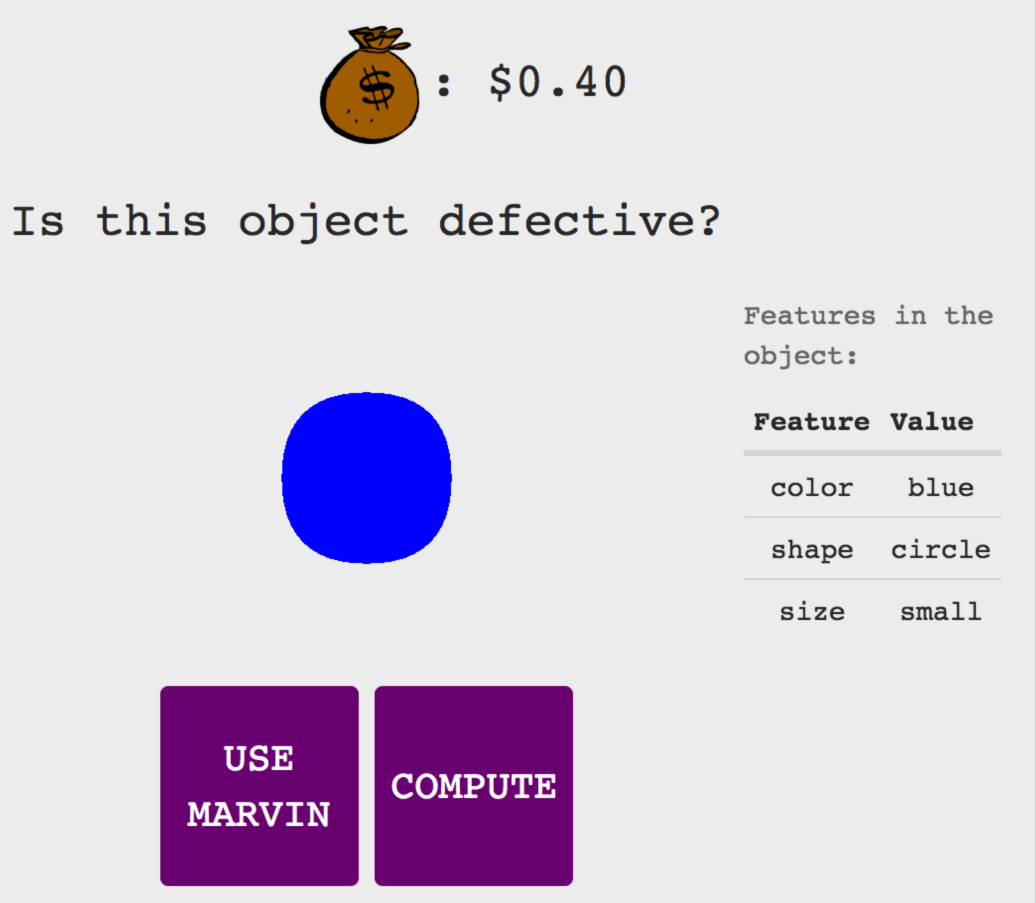
\includegraphics[width=0.8\linewidth]{tutorial-1.png}
    % \vspace{-0.2pc}
    \caption{Screenshot of the \plat\ platform for studying human-AI teams.}
    \label{fig:ui}
    % \vspace*{-1.0pc}
\end{figure}  

How might we study the impact of AI accuracy, updates, compatibility, and mental models on the performance of \name\ teams? Ideally, we would conduct user studies in real-world settings, varying parameters like the length of interaction, task and AI complexity, reward function, and the AI's behavior. All human-subjects research is challenging, but our setting poses special perplexities. Testing in real settings reduces or removes our ability to directly control the performance of the AI. Furthermore, it may largely measure experts' differing experience in the domain, rather than their interactions with the AI.
The importance of mental models for team success
varies among domains and the interaction designed between the AI system and humans. When humans do not have an easy way to validate machine correctness, extracting value out of AI assistance depends on the ability of the human developing a mental model of the AI system. 

To control for human expertise and the centrality of mental modeling, we developed the \plat\ platform, which supports parameterized user studies in an assembly line domain that abstracts away the specifics of problem solving and focuses on understanding the effect of mental modeling on team success. \plat\ is designed such that {\em no} human is a task expert (nor can they become one). In fact, the true label of decision problems in the platform is randomly generated so that people cannot learn how to solve the task. However, humans can learn when their AI assistant, Marvin, succeeds and when Marvin errs. Alongside, the human has access to a perfect problem-solving mechanism, which she can use (at extra cost) when she does not trust Marvin. 


Specifically, \plat\ is a web-based game, whose goal is to make classification decisions for a fixed number of box-like objects.  For each object, the team follows the steps S1-S4 to decide whether the object is ``defective" or not. In S1 a new object appears (\eg,\ blue square), in S2 the AI recommends a label (\eg,\ not-defective), in S3 the player chooses an action (\eg,\ accept or reject the AI recommendation), and in S4 the UI returns a reward and increments the game score. The objects are composed of many features, but only a subset of them are made {\em human-visible}.
For example, visual properties like shape, color, and size are visible, but the contents are not. In contrast, the AI has access to all the features but 
may make errors. At the beginning of the game, users have no mental model of the AI's error boundary. However, to achieve high scores, they must learn a model using feedback from step S4. Figure~\ref{fig:ui} shows a screenshot of the game at step S3. %\Bug{Marco: It's not clear if the user can see the model's prediction before accepting or not.  The screenshot seems to indicate the user can either trust the model blindly or make his own prediction. If this is the case, it's a little contrived. }

\plat\ allows study designers to vary parameters, such as the number of objects, number human-visible features, reward function, AI accuracy, and complexity of perfect mental model (number of clauses and literals in the   error boundary and stochasticity of errors). Further, it enables one to study the effects of updates to AI by allowing changes to these parameters at any time step. In the next section, we use \plat\ to answer various research questions.


\section{Experiments}
We present experiments and results in two parts. First, using our platform, we conduct user studies to understand the impact of mental models and updates on team performance. Second, we simulate updates for three real-world, high-stakes domains and show how the retraining objective enables an explorable tradeoff between compatibility and performance that is not available in the original models.

\noindent {\bfseries User Studies.} In user studies, we hired MTurk workers and directed them to the \plat\ platform.\footnote{Workers were paid on average \$20/hr, over the minimum wage in line with  ethical guidelines for requesters~\cite{dynamo-MT-ethics17}.} We informed them of the purpose of the study and provided a set of simple instructions to familiarize them with the task and the user interface: form a team with an AI, named Marvin, and label a set of 100 objects as ``defective'' or ``not defective''.  
Following \name, to label an object, a worker can either accept Marvin's recommendation, which is initially correct 80\% of the time, or use the ``compute'' option, which is a surrogate for the human doing the task herself perfectly but incurring an opportunity cost.
Table~\ref{tab:payoff} summarizes the reward function  used in our studies. The matrix is designed in a way that it imitates a high-stakes scenario, i.e., the monetary penalty for a wrong decision is much higher than the reward for a correct decision. We found this design choice to be a good incentive for workers to learn and update their mental model on Marvin.  %;  mistakes incur a high penalty, as is typical in high-stakes domains.  ``Computing'' yields a uniform reward of zero, which results from the an increased cost to the human counterbalanced by never making a mistake.  
Note that the expected value of a pure strategy (\eg, always ``Compute"  or always ``Accept," without considering the likelihood of Marvin's correctness) is zero. The only way to get a higher score is by learning when to trust Marvin. While the subjects are told  Marvin's accuracy and the payoff matrix, they can only learn Marvin's error boundary gradually by playing the game.   These design choices allow us to study the impact of mental models while controlling for human problem solving expertise --- every player is able to solve  problems perfectly, at a fixed cost,  using ``compute.''\\


\begin{table}[t]
    \centering
    \begin{tabular}{|c|c|c|}
    \hline
         & Accept & Compute  \\
         \hline
         AI right & \$0.04 & 0 \\
         \hline
         AI wrong & -\$0.16 & 0\\
         \hline
    \end{tabular}
    \caption{Reward matrix for the user studies. To mimic high-stakes domains, penalty for mistakes is set to high. 
    }
    \label{tab:payoff}
\end{table}


\begin{figure*}[t]
  \centering
  \begin{subfigure}[b]{.47\columnwidth}
    \centering
    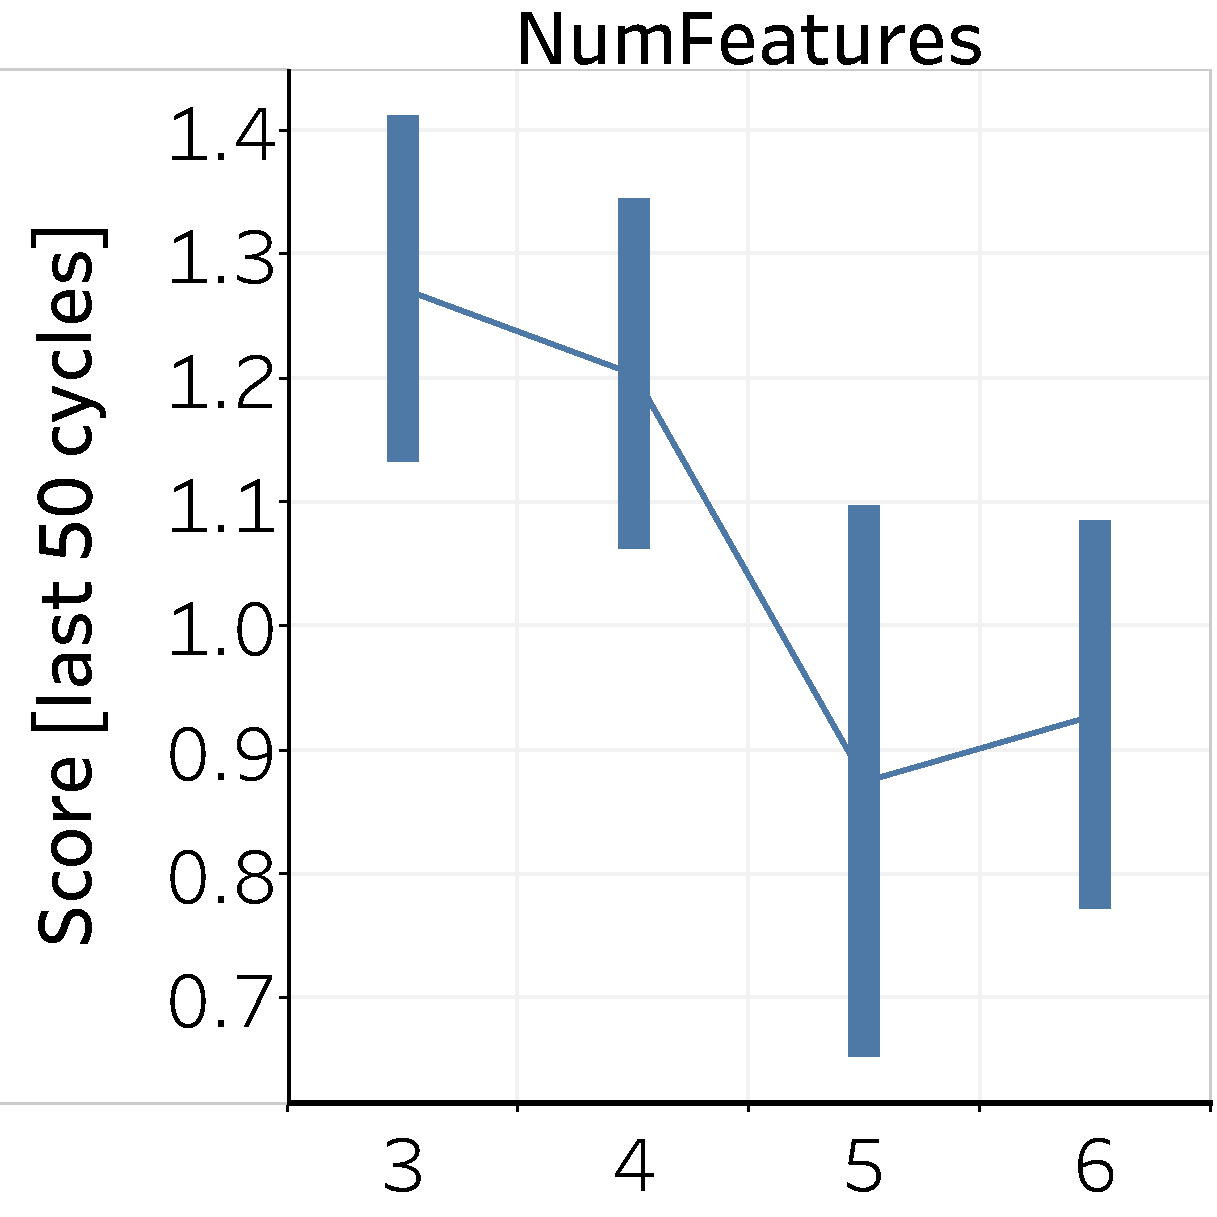
\includegraphics[width=\columnwidth]{2a.pdf}
    \caption{}
    \label{fig:complexity_nonstochastic}
  \end{subfigure}
  \hfill
  \begin{subfigure}[b]{.47\columnwidth}
  \centering
    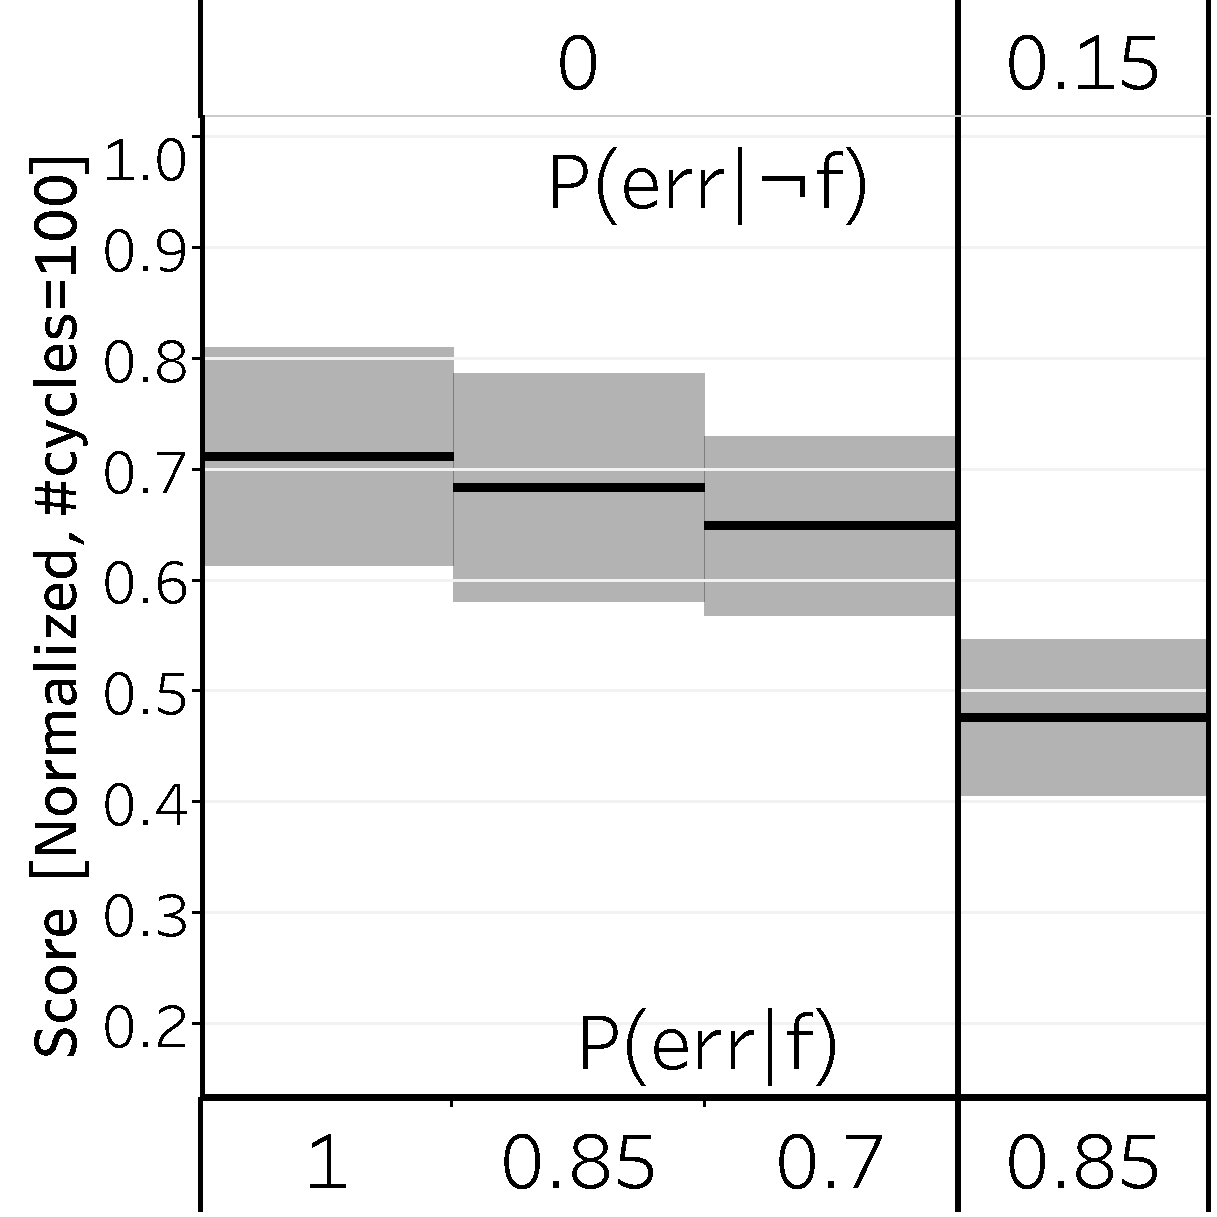
\includegraphics[width=\columnwidth]{2b.pdf}
    \caption{}
    \label{fig:complexity_stochastic}
  \end{subfigure}
    \hfill
  \begin{subfigure}[b]{0.47\columnwidth}
  \centering
    \centering
    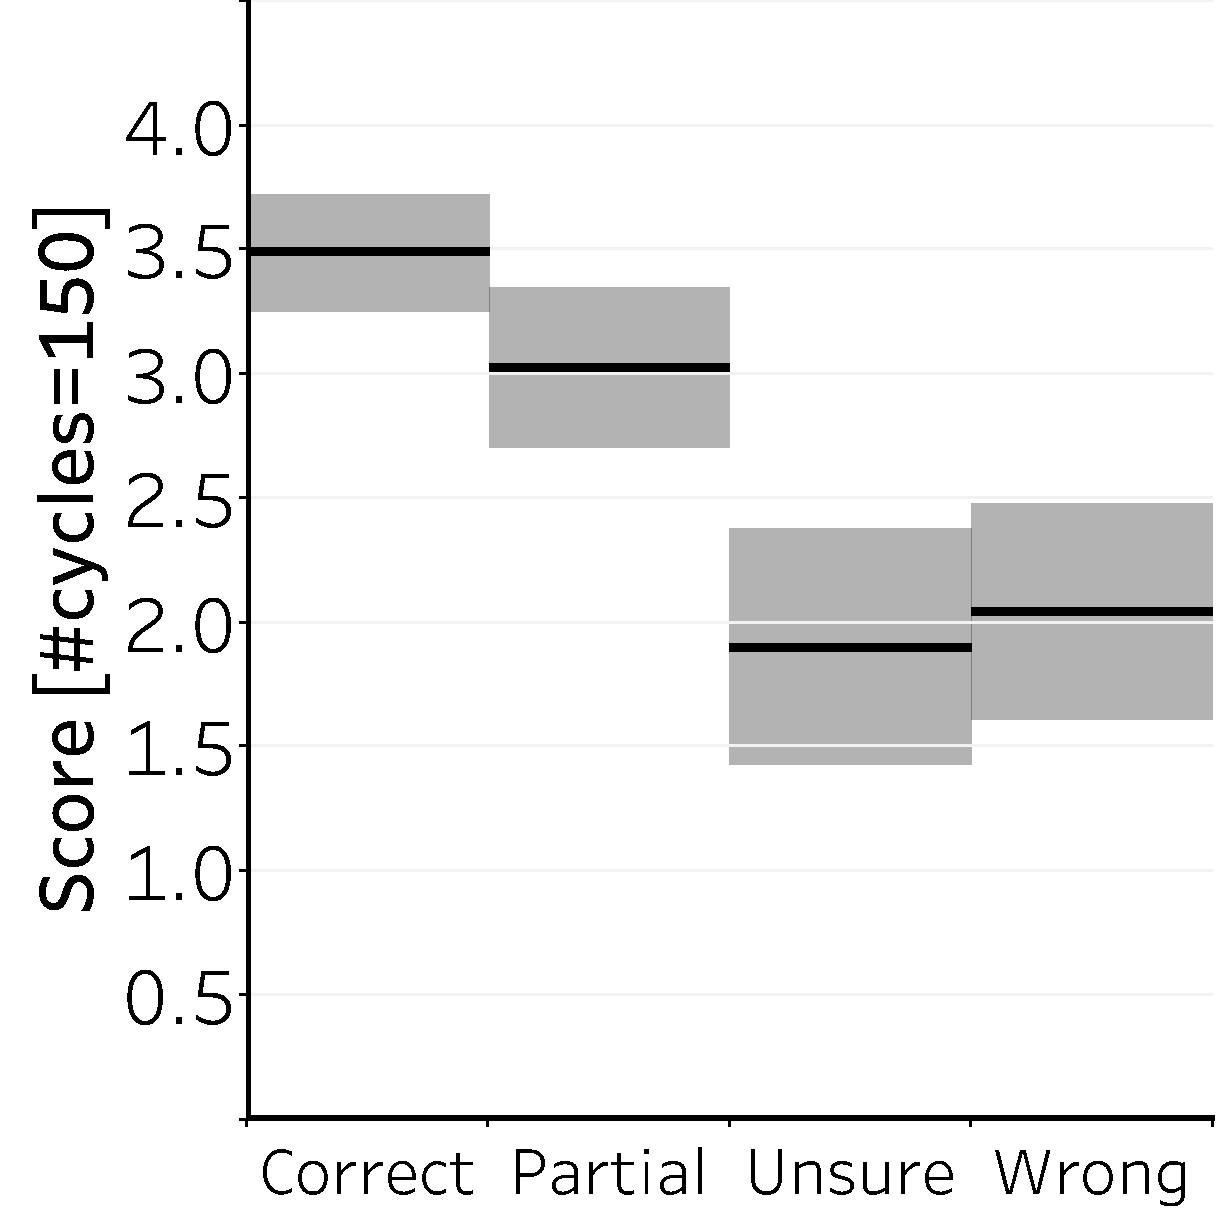
\includegraphics[width=\columnwidth]{wsl.pdf}
    \caption{}
    \label{fig:wsl}
  \end{subfigure}
  
  \caption{(a) Team performance decreases as we increase the number of human-visible features. (b) Team performance decreases with the stochasticity of errors. The decrease is much higher for two-sided errors. (c) Better mental models result in higher team performance. Wrong and Unsure mental models have the lowest performance. 
  }
  \label{fig:complexity}
\end{figure*}

\begin{figure}[t]
  \centering
    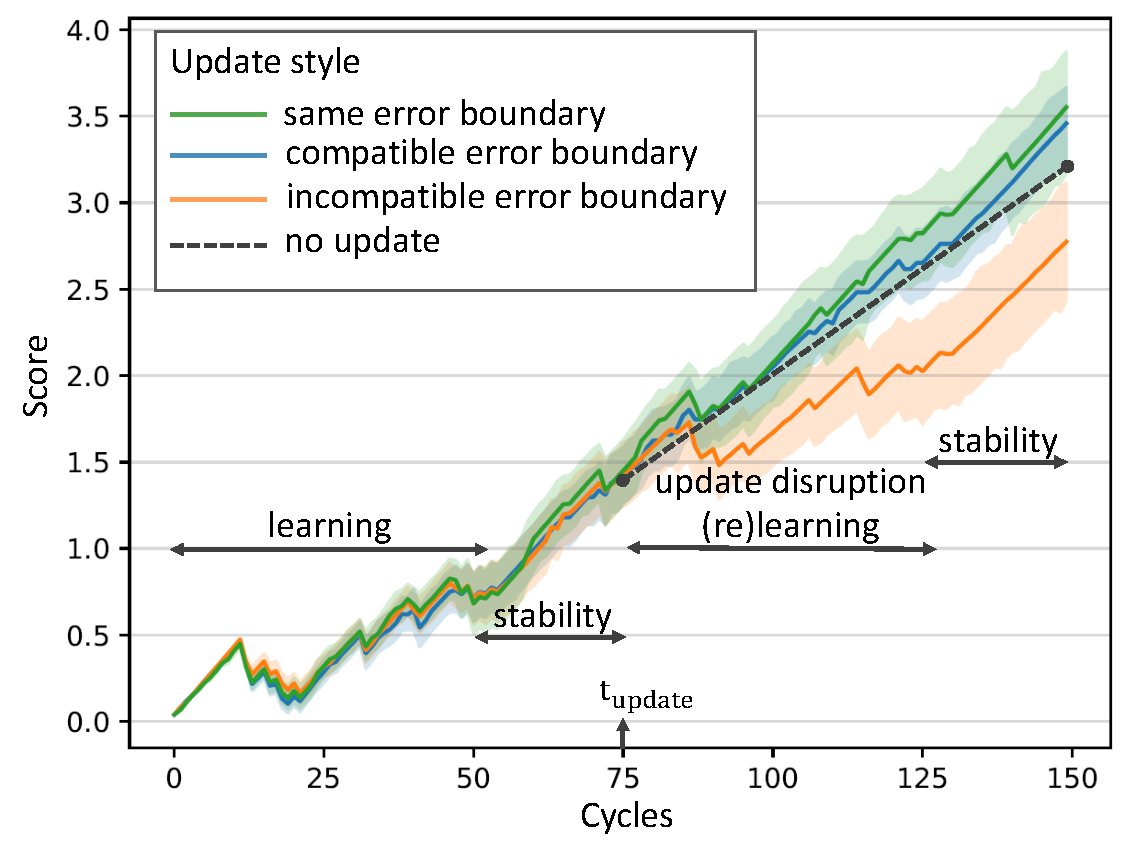
\includegraphics[width=\columnwidth]{update_study.pdf}
    \caption{Team performance for different update settings. Compatible updates improve team performance, while incompatible updates hurt team performance  despite improvements in AI accuracy.}
    \label{fig:updateExp}
\end{figure}

\noindent {\bfseries Q1: }{\em Do better mental models of AI lead to higher team performance?}\\
\noindent To answer this, we conducted human studies that measured team performance across different conditions of complexity of task and error boundary.
For each condition, we hired 25 MTurk workers, and filtered spammers by deleting data from workers in the bottom quartile.  
We varied the task complexity by varying the number of human-visible features. The complexity of error boundary $f$, expressed as a logical formula, is varied by changing the number of conjuncts and literals in $f$. For example, we tried one conjuncts containing two literals, one conjunct with three literals, and two conjuncts with two literals. 
Since many features can be used as literals,  we chose them randomly to create different but isomorphic error boundaries. For example, worker A gets $f_A = (blue \cap square)$ and worker B gets $f_B = (red \cap circle)$.
Figure~\ref{fig:complexity_nonstochastic} shows that, for one conjunct and two literals, team performance decreases with the number of features. We observed a similar behavior for other error boundaries (results omitted for space), and for the rest of these studies we set the number of conjuncts to one.
 Figure~\ref{fig:complexity_nonstochastic} shows that, as the number of features increases, team performance decreases because it becomes harder to create a mental model.

Next, we conducted a study (Figure~\ref{fig:complexity_stochastic}) to understand the impact of {\em stochasticity} in the error boundary on team performance.  
Stochasticity is defined using two conditional probabilities: $P(\err | f)$ and $P(\err | \neg f)$. That is, the probability of error if $f$ is satisfied, and if it is not satisfied. To vary stochasticity, we chose the following four pairs of probabilities: (0.7, 0), (0.85, 0), (1.0, 0), and (0.85, 0.15). For the first three pairs, the errors are ``one-sided'': since $P(\err|\neg f)$ is 0, the classifier makes a mistake only if the formula is satisfied. In the last pair, errors are ``two-sided'': with a probability of 0.15, the classifier makes a mistake even if the formula is not satisfied.
We fix the number of features to three and the number of literals to two.
Figure~\ref{fig:complexity_stochastic} shows that as errors become more stochastic, it becomes harder to create a mental model, deteriorating team performance. The $y$-axis shows the score normalized by the score of the optimal policy because, as we vary stochasticity, the optimal policy's score changes.

Finally, in order to have a closer view of the quality of the workers' mental models, we ask them to self report when they thought Marvin was wrong. We manually labeled these reports as correct, partial, unsure, and wrong, without looking at their team performance. The label denotes how the worker's mental model compared to the true error boundary $f$. For example, correct denotes that the mental model and $f$ were the same, wrong denotes no match, partial denotes an incomplete match, and unsure denotes that the worker was skeptical of their mental model. Figure~\ref{fig:wsl} compares team performance on these groups. Workers with the correct mental model score the highest, followed by workers with a partially correct model. These observations confirm that better mental models contribute positively to team performance.\\


\noindent {\bfseries Q2: }{\em Do more compatible updates lead to higher team performance than incompatible updates?}\\
\noindent To study the impact of updates, we set the number of cycles to 150, and at the 75th cycle, update the classifier to a version that is 5\% more accurate (80\% $\rightarrow$ 85\%). Then, we divide the participants into three groups: same error boundary,
compatible error boundary, and incompatible error boundary. The same error boundary group receives an update improving accuracy, but the  error boundary is unchanged. For the two other groups, the number of literals (features) in the error boundary changes from two to three. The update for the compatible error boundary group introduces no new errors; for example, if before the update the error boundary was $blue \cap square$, after the update it may change to $small \cap blue \cap square$. For the incompatible error boundary group, the error boundary introduces new errors violating compatibility. Figure~\ref{fig:updateExp} summarizes our results. We also show the performance of workers if no update was introduced (dashed line). It uses the no-update setting from experiments in Q1, and extrapolates from there assuming that the worker's mental model is already stable at the 75th cycle, meaning that the human-AI team has reached the maximum performance for the original setting and no further improvements are expected. The graph demonstrates two main findings on the importance of compatibility. First, a more accurate but incompatible classifier  results in lower team performance than a less accurate but compatible classifier (no update). Second, compatible updates improve team performance. Moreover, the figure shows different stages during the interaction: the user learning the original error boundary, team stabilizes, update causes disruption, and performance stabilizes again. A central insight in the update stage is that the incompatible error boundary condition sacrifices the team score while workers have to relearn the new boundary. This insight shows that compatible updates not only improve team performance but they can also reduce the cost of retraining users after deploying system updates.  


\subsection{Experiments with  High-Stakes Domains}
\noindent {\bfseries Datasets.} To investigate whether a tradeoff exists between  performance and compatibility of an update, we simulate updates to classifiers for three domains: recidivism prediction (Will a convict commit another crime?)\cite{angwin2016machine}, in-hospital mortality prediction (Will a patient die in the hospital?) \cite{johnson2016mimic,harutyunyan2017multitask}, and credit risk assessment (Will a borrower fail to pay back?)\footnote{\url{https://community.fico.com/s/explainable-machine-learning-challenge}}. We selected these high-stakes domains to highlight the potential cost of mistakes caused by incompatible updates in human-AI teams.\\\\

\begin{table}[t]
\footnotesize
\centering
\begin{tabular}{|l|l|c|c|c|}
\hline
Classifier & Dataset                         & ROC $\hone$ & ROC $\htwo$ & $\compatscore(\hone, \htwo)$ \\
\hline
LR & Recidivism       &   0.68 &        0.72     &   0.72               \\
& Credit Risk          &   0.72     &    0.77    &   0.66              \\
& Mortality    &    0.68 &    0.77    &    {\bf 0.40}                    \\
\hline
MLP & Recidivism   &   0.59     &     0.73   &     0.53                    \\
& Credit Risk     &  0.70   &    0.80    &     0.63                     \\
& Mortality &       0.71 &     0.84   &     0.76            \\
\hline
\end{tabular}
\caption{\label{tab:score} Although training on a superset of data increases classifier performance, compatability can be suprisingly low.}
\end{table}


\begin{figure*}[t]
    \centering
    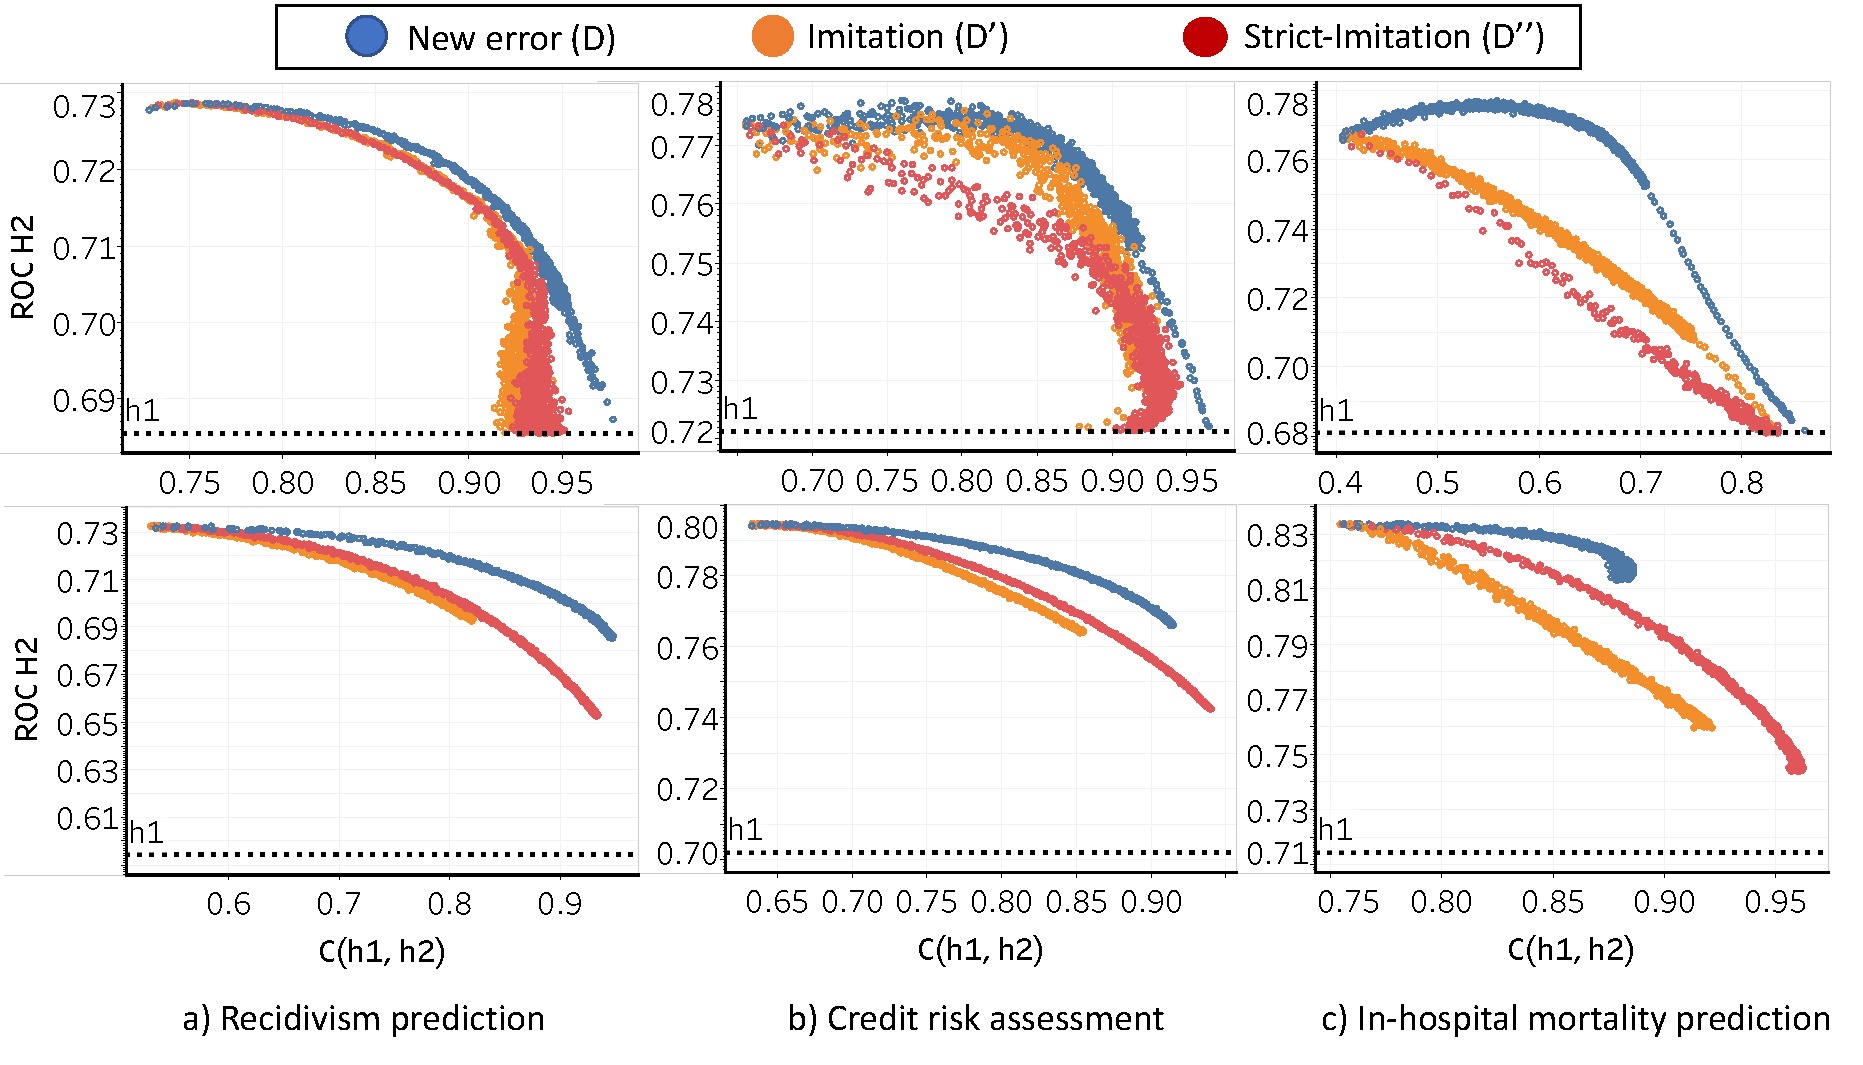
\includegraphics[width=0.9\linewidth]{figure5.pdf}
    \caption{Performance vs. compatibility for a logistic regression and multi-layered perceptron classifiers. The reformulated training objective ($\lossbc$) offers an explorable performance/compatibility tradeoff, generally more forgiving during the first half of the curves. The training objective based on new-error dissonance performs the best, whereas the ones based on imitiation and strict-imitation dissonance perform worse since they imitate probabilities of a less accurate, and less calibrated model ($\hone$).}
    \label{fig:diss}
\end{figure*}
\noindent {\bfseries Q3: }{\em Do current ML classifiers produce compatible updates?}\\
\noindent For this experiment, we first train a classifier $\hone$ on 200 examples and note its performance. Next, we train another classifier $\htwo$ on 5000 examples
% \Bug{justify why we used such small number of examples: DW i don't see a way to do so without increasing our risk. I'd just remove the bug}
and note its performance and compatibility score. We train both classifiers by minimizing the negative log loss. Table~\ref{tab:score} shows the performance (area under ROC) and compatibility averaged over 500 runs for logistic regression (LR) and multi-layer perceptron (MLP) classifiers. We find that training $\htwo$ by just minimizing log loss does not ensure compatibility. For example, for logistic regression and the in-hospital mortality prediction task, the compatibility score is as low as 40\%.  That is, 60\% of the instances where $h_1$ was correct are now violated.\\


\noindent {\bfseries Q4: }{\em Does there exist a tradeoff between the performance and the compatibility of an update to AI?}\\
\noindent For Q4 (and Q5), we learn the second classifier $\htwo$ by minimizing $\lossbc$. As $\lossbc$ depends also on the first classifier, we make its prediction available to the learner. We vary $\lambdabc$ and summarize the resulting performance and compatibility scores across different datasets for the logistic regression and multi-layer perceptron classifiers in Figure~\ref{fig:diss} and for different definitions of dissonance (discussed in Q5). 
The figure shows that there exists a tradeoff between the performance of $\htwo$ and its compatibility to $\hone$. This tradeoff is generally more flexible (flat) in the first half of the curves. This shows that, at the very least, one can choose to train via $\lossbc$ and deploy a more compatible update without significant loss in accuracy. Although such updates are not fully compatible, they might still be relevant if the update is supported by efficient explanation techniques that can help users to better understand how the model has changed. In these cases, a more compatible update would also reduce the effort of user (re)training. In the second half, the tradeoff becomes more evident. High compatibility can sacrifice predictive performance. Look-up summaries similar to graphs shown in Figure~\ref{fig:diss} are an insightful tool for ML developers that can guide them select an accurate yet compatible model based on the specific domain requirements. \\

\noindent {\bfseries Q5: }{\em What is the relative performance of the different dissonance functions?}\\
 Figure~\ref{fig:diss} compares the performance of the new-error dissonance function ($\dissonance$) with the imitation-based dissonances ($\dissonance'$  and  $\dissonance''$). As anticipated, $\dissonance$ performs  best on all  three domains. The definitions inspired by model distillation, $\dissonance'$ and $\dissonance''$,  assume that \hone\ is calibrated, and more accurate. Therefore, $\htwo$ needs to remain faithful to only the correct regions of a less accurate model $\hone$. If these assumptions are violated, $\htwo$ overfits to non-calibrated confidence scores of $\hone$, which hurts performance.


\section{Discussion and Directions}


The AI-assisted human decision-making problem assumes that there are instances for which the AI is more efficient (\eg,\ higher accuracy, faster, or low resource usage), and the human can recognize when the AI is capable of doing so. Earlier, we discussed that one way for humans to recognize when to follow the AI's recommendations is by creating mental models. However, depending on the domain and the type of interaction design, the importance of mental modeling for team performance may vary. For example, if the human can quickly validate the correctness of the recommendation, or the human expertise improves over time to leave no room for machine contribution, then mental modeling may not be needed. Otherwise, the accuracy of the mental model limits team performance. Thus, compatibility of updates becomes an essential determinant of team performance, and developers should factor it in system design supported by guiding tools exploring the performance/compatibility tradeoff. 
 
Varying the value of $\lambdabc$ results in numerous models on the performance/compatibility spectrum. The decision to select the appropriate model depends on several factors, including the user ability to create a mental model, the cost of disruption, and whether there exist other alternative approaches for minimizing disruption caused by updates. For example, if the cost of disruption (both the cognitive cost and mistakes) is high, then we may use a high value for $\lambdabc$. A more formal approach would be to set $\lambdabc$ algorithmically. For example, a $\lambdabc$ could be selected to maximize expected utility expressed using a computational user model and future rewards.

A developer can use other complementary approaches to minimize disruption caused by low compatibility. One approach is to retrain the user, for example, by leveraging mechanisms from interpretable AI to explain the updated model to users or to explain differences between \hone\ and \htwo. However, this may not always be practical: 
(1) in practice, developers may push updates frequently, and since re-training requires user’s additional time and effort, it may not be practical to subject experts to repeated re-training; 
(2) updates can arbitrarily change the decision boundary of a classifier, and as a result, require the user to re-learn a large number of changes;
(3) re-training requires the developers to create an effective curriculum or generate a “change summary” based on the update. It is often impossible to compute such summaries in a human-interpretable way.
For example, explaining the changes to a self-driving car may require the challenging task of mapping the feature representation used by the car (myriad of sensor data) to human-interpretable concepts.
Nevertheless, backward compatibility does not preclude retraining; these techniques are complementary to each other. In fact, more compatible updates can be an efficient mechanism to simplify the re-training process by minimizing the divergence between two models deployed consecutively. Yet another complementary approach is to share the AI's confidence in the prediction. Well-calibrated confidence scores can help a user to decide when or how much to trust the system. Unfortunately, confidence scores of ML classifiers are often not calibrated~\cite{nguyen2015deep} or a meaningful confidence definition may not exist due to the complexity of the task.

We formalized compatibility in terms of differences in model recommendations before and after an update, independent of mental models of users. An important future direction is to develop computational models of how people create and update mental models, and condition on the personalized experiences and cognitive capabilities of each user, drawing upon general findings about how people learn about phenomena via observation~\cite{reber1989implicit}. While this work distills trust as the essence of teamwork and presented results are applicable to a variety of use cases, promising extensions include developing blended studies in the real world that combine both factors of human problem solving and learned trust in AI. 


\section{Related Work}


Prior seminal work explored the importance of mental models for achieving high performance in group work~\cite{grosz1999evolution}, human-system collaboration (Rouse \etal\ 1992), and interface design~\cite{carroll1988mental}. Our work builds upon these foundations and studies the problem for \name.
Other work~\cite{hoff2015trust} highlights the connection between mental models and trust in systems.
While many ``layers'' of trust exist, our work focuses on {\em learned trust}, which is built upon context and past experiences~\cite{marsh2003role}.
Previous work \cite{zhou2017effects} investigated factors that affect user-system trust, e.g., model uncertainty and cognitive load. The platform proposed in this work enables human studies that can analyze the effect of such factors.


The field of software engineering also considers the problem of backward compatibility, seeking to design components that, after  updates, remain compatible with a larger software ecosystem~\cite{bosch2009software,spring2005techniques,tsantilis2009method}.
Machine learning research has explored related notions. {\em Stability} expresses the ability of a model to not significantly change its predictions given  small changes in the training set~\cite{bousquet2001algorithmic}. {\em Consistency}, which has application in ML fairness, is a property of smooth classifiers, which output similar predictions for similar data points
~\cite{zhou2004learning}. 
\emph{Catastrophic forgetting} is an anomalous behavior of neural network models that occurs when they are sequentially trained to perform multiple tasks and forget to solve earlier tasks over time~\cite{kirkpatrick2017overcoming}. 
While  these concepts are fundamental for analyzing changing trends in continuously learned models, they do not consider human-AI {\em team} performance nor prior user experience. Related to our proposed retraining objective is the idea of \emph{cost-sensitive} learning~\cite{elkan2001foundations}, where different mistakes may cost differently; for example, false positives may be especially costly. However, in our case, the cost also depends on the behavior of the previous model $\hone$.

\section{Conclusions}
    We studied how updates to an AI system can affect human-AI team performance and introduced methods and measures for characterizing and addressing the compatability of updates. We introduced \plat, a platform for measuring the effect of AI performance and the effect of updates on team performance. Since humans have no experience with \plat's abstract game, the platform controls for human problem-solving skill, distilling the essence of mental models and trust in one's AI teammate.
    Using \plat, we presented experiments  demonstrating how an update that makes an AI component more accurate can still lead to diminished human-AI team performance. % when updates break the expectations and trust of the human user.
    We introduced a practical re-training objective that can improve the compatibility of updates. 
    Experiments across three data sets show that our  approach creates updates that are more compatible, while maintaining high accuracy. 
    Therefore, at the very least, a developer can choose to deploy a more compatible model without sacrificing performance. 
    
    

\section{Acknowledgments}
We thank  M.  Ribeiro,  S.  Tan,  X.
Zhang,  R.  Caruana,  M.  Czerwinski,  J.  Suh,  M.  Joshi,  J.
Bragg, and anonymous reviewers for helpful feedback. This work was
was supported by Microsoft Research, ONR grant N00014-18-1-2193, the future of Life foundation and the WRF/Cable Professorship.

% References and End of Paper
% These lines must be placed at the end of your paper
\bibliography{main}
\bibliographystyle{aaai}
\end{document}
